In order to meet the problem identified in \autoref{sec:introduction}, GitSlice has been implemented as a Python 3 application.
GitSlice is configured using a YAML file, which defines the exact parameters of commits be selected, the analysis tool to be run and the location of output from the analysis tool.
The analysis tool is given as a Singularity image (see \autoref{subsec:singularity}).
GitSlice supports a different analysis tool depending on the version of the project---for example, if a Python project is currently written using Python 3 but a previous version required Python 2, a Python 2 container can be used for older versions.
Similarly, the command to invoke the analysis tool is configurable based on the version---if for example the location of the main script has changed, a command that invokes test coverage may be different depending on the version.

GitSlice can run across multiple nodes in an HPC cluster.
When executed, GitSlice will inspect the repository to identify the commits to be analysed on the primary node (the node with an ID of \codeword{0}) and the commits are then distributed across all the nodes allocated to GitSlice (see \autoref{subsec:mpi}) each of which will begin analysing the commits allocated to it.
Each node will clone the repository and represent it as virtual filesystem, the commit to be analysed will be mounted on the analysis container and the appropriate command (depending on the version) will be run.
GitSlice then presents the files as they existed at that commit to the analysis container by binding the appropriate subdirectory from the virtual filesystem to the container.
The output from the analysis container is then saved to the output directory defined in the configuration file.

\subsection{Parallel Execution using MPI}
\label{subsec:mpi}

GitSlice uses MPI to allow for multiple nodes to work together to analyse the repository.
One instance of GitSlice will be the ``primary'' instance, with $ 0 $ or more ``secondary'' instances which await a commit ID to perform analysis on.
Upon initialisation of GitSlice, the primary instance will analyse the repository to identify the commits to be analysed.
Each instance of GitSlice creates its own directory inside the output directory identified by a UUID generated on initialisation.
This enables any amount of instances of GitSlice to work on analysing the repository without overwriting work from another instance.
The work is evenly divided among all instance of GitSlice---for example, if there are $ 5 $ instances with $ 25 $ commits to be analysed then each instance will analysed $ 5 $ commits.
Multiple threads are also used to allow for each instance to analyse multiple commits simultaneously.
For example, if there are $ 5 $ instances each with $ 5 $ threads then 25 commits will be analysed simultaneously.
\autoref{fig:mpi_diagram} illustrates this visually.

\begin{figure*}[ht]
	\centering
	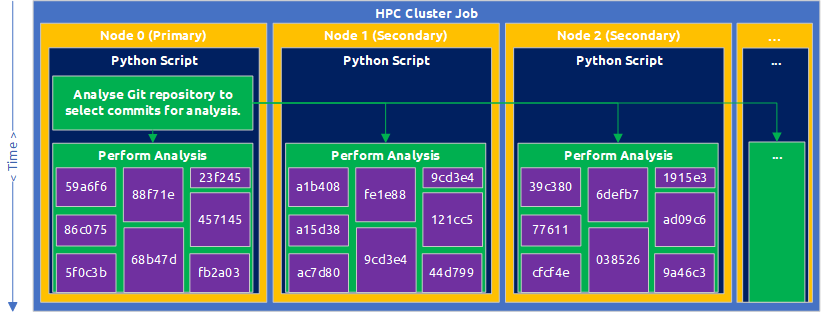
\includegraphics[width=\textwidth]{images/mpi_diagram}
	\caption{Illustration of how GitSlice operates using MPI across multiple nodes.}
\label{fig:mpi_diagram}
\end{figure*}

\subsection{Accessing Git Commits Through a Virtual Filesystem}
\label{subsec:filesystem}

GitSlice needs to recreate the files of the project being analysed as they existed at a particular commit in order to bind this to the analysis container.
Multiple commits cannot be checked out at once so the initial implementation of GitSlice created a copy of the repository for each analysis with the appropriate commit checked out in a detached \codeword{HEAD} state (this means a commit has been checked out directly, as opposed to a branch).
This caused quite a lot of overhead as the entire repository is deleted and copied over and over again.
To prevent this, RepoFS\cite{repofs} was used.
RepoFS is a Python project which exposes the repository as a virtual filesystem.
When run, RepoFS will create a filesystem which contains a directory named \codeword{commits-by-hash/} among others.
Within this directory is a subdirectory for each commit, named using the commit ID of the commit.
Inside each of these commit directories is the project as it existed at that commit.

Each parallel instance mounts its own virtual filesystem as HPC clusters typically use a network filesystem to keep a consistent filesystem across nodes.
Mounts are not shared across the network so each instance must mount its own virtual filesystem.
When an instance is finished analysing all the commits assigned to it, it will bring the mount down.

\subsection{Analysis Using Singularity Containers}
\label{subsec:singularity}

Typically, to run an analysis application it would be necessary to install all the required dependencies which is not an option in HPC cluster environments where installing arbitrary tools is usually not allowed for security reasons.
A solution to this is containers which encapsulate all the required dependencies to run an application within an isolated environment.
Containers utilize the same kernel as their host and in this way they differ from virtual machines---this also makes containers much more lightweight than virtual machines.
Singularity is a container platform designed for use in HPC environments~\cite{singularity}.
It supports Docker images, the most widely used containerisation platform.
Support for Docker images enables a very wide variety of images to be executed, Docker Hub for example currently contains over 100,000 images.

When running an analysis tool, the use of containers also allows for the complete isolation of the filesystem running the analysis tool.
This is important as it prevents multiple executions of an analysis tool from writing to the same files (for example, outputting analysis reports to the same location).

\subsection{Configuration}
\label{subsec:configuration}

When run, GitSlice accepts three arguments; the location of a configuration file, the level of logging to use (where logging output is one of the following: debug, info, warning, error and critical) and if dry run is enabled (in dry run mode GitSlice will not perform analysis but instead will output the commits which would have been selected based on the configuration file).
The configuration file specifies the following settings:

\begin{itemize}
    \item \textbf{Output Directory}: the directory in which the output from each commit will be saved as a text file to.
    \item \textbf{Output Format}: the format of the output file, for example each file can be named by the time of the commit and the commit ID with an underscore to separate them.
          The time of the commit here refers to the commit time as opposed to author time.
          Output files is saved as a .txt file.
    \item \textbf{Temp Directory}: the directory to use for creating a temporary copy of the repository.
          It is recommended this location is stored locally as opposed to a network location for performance.
          It is not necessary for files in the directory to be able to be accessed by all nodes, but all nodes must be able to create directories at this location.
    \item \textbf{Rsync To Temp}: the virtual filesystem is read only so the container cannot modify the or create files.
          GitSlice provides a feature which will use \codeword{rsync} to copy files from the directory containing the files of the commit to be analysed to a temporary directory to enable the analysis tool to modify and create files.
          This feature is enabled when this option is set to true.
    \item \textbf{Mount Directory Name}: the name of the directory inside the temporary directory where the virtual filesystem will be mounted at.
    \item \textbf{Repo Directory Name}: the name of the directory inside the temporary directory which will contain the repository.
    \item \textbf{Git Repository Type}: indicates if the repository is local or remote, remote repositories will be cloned into the temporary directory and local repositories will be copied into it.
    \item \textbf{Git Repository Source}: the source of the repository, an absolute or relative path for local repositories and a full URI for remote repositories.
    \item \textbf{Analysis}: this block contains a list of commits IDs which contain \textbf{Image} and \textbf{Command} values.
          When that commit exists as a parent (not necessarily a direct parent) of the commit, the \textbf{Image} and \textbf{Command} values will be used.
          Where multiple commits listed in this section are parents, the most recent parent's \textbf{Image} and \textbf{Command} values will he used.
    \item \textbf{Starting Point} and \textbf{Stopping Point}: these options provide Git objects (commits, tags, branches etc.) for which the ancestry path between them will be the commits which are selected for analysis.
    \item \textbf{Git Rev List Args}: GitSlice uses the \codeword{git-rev-list} command to find the ancestry between the \textbf{Starting Point} and \textbf{Stopping Point}, this block contains arguments which can be passed to this command.
          This enables a reduction in the commits which are analysed based on a large amount of properties---for example, this allows for selecting only commits created by certain author(s), commits which were committed or authored before or after a certain date, only merge commits to be selected or only non-merge commits to be selected and many more.
          The manual pages for the \codeword{git-rev-list} command provide a thorough explanation of all the options available here.
    \item \textbf{Additional Filters}: finally, GitSlice also provides additional commit filtering options which are not provided by \codeword{git-rev-list}, this includes limiting to a certain amount of commits, skipping a certain amount of commits (for example, select one and then skip 3 commits before selecting the next), selecting only commits with certain amounts of files changed, insertions and deletions, selecting only commits which change particular file types and selecting commits based on a minimum amount of time between commits (i.e.\ one commit every 30 days).
\end{itemize}
